\documentclass{llncs}
\usepackage{makeidx}  % allows for indexgeneration
\usepackage{acronym}
\usepackage[numbers]{natbib}
\bibliographystyle{splncs03} 

\usepackage{nameref}
\usepackage{hyperref}
%\usepackage[hyphens]{url}
%\usepackage[hyphenbreaks]{breakurl}
\usepackage[USenglish]{babel}
\usepackage[T1]{fontenc}
\usepackage{amsmath}
\usepackage{amssymb}
\usepackage{pslatex}
%
\DeclareMathOperator{\tr}{tr}
\DeclareMathOperator{\argmax}{argmax}
\DeclareMathOperator{\argmin}{argmin}
\DeclareMathOperator{\diag}{diag}
\DeclareMathOperator{\dist}{dist}
\DeclareMathOperator{\const}{Const.}

\usepackage{graphicx}
%
%\tableofcontents
%
\mainmatter              % start of the contributions
%
\graphicspath{{../Figures/}}

\begin{document}

\title{Simultaneous segmentation and distortion correction on diffusion weighted MR using shape priors}
%%
\titlerunning{Simultaneous segmentation and distortion correction on DWI}  % abbreviated title (for running head)
%                                     also used for the TOC unless
%                                     \toctitle is used
%
\author{Oscar Esteban\inst{1,2} \and
        Alessandro Daducci \inst{2} \and
		Meritxell Bach-Cuadra \inst{2,3} \and
        Jean-Philippe Thiran \inst{2,3} \and
        Andr\'es Santos \inst{1} \and
        Dominique Zosso \inst{2,4}}
%
\authorrunning{Oscar Esteban et al.} % abbreviated author list (for running head)

\institute{Biomedical Image Technologies (BIT),
ETSI Telecomunicaci\'on - Universidad Polit\'ecnica de Madrid
and CIBER-BBN, \\
Av. Complutense 30, E-28040 Madrid, Spain\\
\email{phd@oscaresteban.es},\\
% WWW home page:
%\texttt{http://users/\homedir iekeland/web/welcome.html}
\and
Signal Processing Laboratory (LTS5),
\'Ecole Polytechnique F\'ed\'erale de Lausanne (EPFL)\\
EPFL STI IEL LTS5, Station 11, CH-1015 Lausanne, Switzerland
\and
Dept. of Radiology, University Hospital Center (CHUV) and University of Lausanne (UNIL) \\
Rue du Bugnon 46, CH-1011 Lausanne, Switzerland
\and
Department of Mathematics, 
University of California, Los Angeles (UCLA) \\
520 Portola Plaza, Box 951555, Los Angeles, CA 90095-1555, USA
}


\maketitle              % typeset the title of the contribution

% List of acronyms used in the text
\acrodef{mr}[MR]{Magnetic Resonance}
\acrodef{mri}[MRI]{Magnetic Resonance Imaging}
\acrodef{dwi}[DWI]{Diffusion Weighted Imaging}
\acrodef{dti}[DTI]{Diffusion Tensor Imaging}
\acrodef{t1}[T1]{T1-weighted}
\acrodef{t2}[T2]{T2-weighted}
\acrodef{csf}[CSF]{cerebrospinal fluid}
\acrodef{wm}[WM]{White Matter}
\acrodef{gm}[GM]{Grey Matter}
\acrodef{epi}[EPI]{echo-planar imaging}
\acrodef{fa}[FA]{fractional anisotropy}
\acrodef{md}[MD]{mean diffusivity}
\acrodef{acwe}[ACWE]{Active Contours without edges}

\begin{abstract}
In whole-brain connectivity analysis of diffusion MRI (dMRI) data,
an accurate delineation of the white-matter and grey-matter surfaces is required.
While high-standard segmentation is readily available for anatomical MRI, such 
as T1-weighted, dMRI typically have lower resolution and severe 
geometrical distortions. We propose a dMRI segmentation-registration framework 
that exploits the detailed anatomy extracted from anatomical MRI as shape-prior.
We use an ``active contours without edges''-like model to look for a deformation
field that optimally maps the shape prior on the multivariate features 
in diffusion space. This joint approach reflects the intrinsic coupling of 
segmentation and distortion correction. Complementary, a precise and consistent
cortical parcellation on dMRI is straightforward by projection from T1 space. Thus,
we expect to improve the reliability and robustness of the resulting connectivity 
networks and their comparability within and across subjects. First results 
on synthetic datasets and simulated dMRI confirm the effectiveness of our approach.
\keywords{ magnetic resonance, diffusion weighted imaging, distortion correction, segmentation, registration, shape priors, connectomics, echo planar imaging
           }
\end{abstract}


\section{Introduction}
\label{sec:introduction}
%
\ac{dwi} is a widely used family of \ac{mr} techniques
\citep{sundgren_diffusion_2004} which recently has accounted for a growing
interest in its application to whole-brain structural connectivity analysis.
This emerging field, coined in 2005 as \emph{\ac{mr} Connectomics}
\citep{hagmann_diffusion_2005,sporns_human_2005}, currently includes a
large amount of imaging techniques for acquisition, processing, and analysis
specifically tuned for \ac{dwi} data.

The whole-brain connectivity analysis has given rise to some challenges
towards reliable structural information
about the neuronal tracts from \ac{dwi} \cite{johansen-berg_using_2009,
jones_white_2012}. The earlier stages of these
processing pipelines generally include two necessary steps, brain tissue
segmentation on the diffusion space and the correction of geometrical
distortions inherent to the imaging techniques \citep{hagmann_mr_2012}.

In this work, we will refer as brain tissue segmentation to the precise
delineation of the \ac{csf}-\ac{gm} and \ac{gm}-\ac{wm} interface surfaces.
This segmentation is an processing step on which strongly rely further
tasks. In tractography, a high-standard \ac{wm} mask is required. Otherwise,
there is an important risk for the algorithm to lose fiber bundles. This
requirement is usually solved in practice by plainly thresholding the 
\ac{fa}, a well-known scalar map derived from \ac{dwi} which depicts 
the isotropy of water diffusion inside the brain. 
A precise location of the
\ac{gm}-\ac{wm} surface is also essential in the final steps to
achieve a consistent parcellisation of the cortex to represent the nodes 
of the output network. This parcellisation is generally defined in a 
high-resolution and better understood structural \ac{mri} of the same 
subject (e.g. \ac{t1} and/or \ac{t2} weighted acquisitions). %Conversely, this problem is resolved with non-linear registration of a structural \ac{mri} of the subject to the \ac{dwi} data. 
Even though some efforts have addressed
the study of the robustness of tractography with respect to intra-subject variability
\cite{wakana_reproducibility_2007,heiervang_between_2006}, these results are restricted to some regions of the brain, only. Therefore, robust
and precise segmentation methods are required in the whole-brain application. 

The \ac{dwi} data is usually obtained with \ac{epi}
acquisition techniques, that often suffer from severe distortions due to 
local field inhomogeneities. Generally, it is appreciated in the anterior
part of the brain, along the phase-encoded direction. Some methodologies have
been developed and generically named as \emph{\ac{epi}-unwarp} techniques
\cite{holland_efficient_2010,hsu_correction_2009,jezzard_characterization_2005,
reber_correction_2005}. These methods usually 
require the extra acquisition of the magnitude and phase of
the field (``field-mapping''), a condition which is not always met. Some other 
methodologies do not make use of the field-mapping, compensating the distortion
with non-linear registration from structural \ac{mri} or other means
\citep{andersson_modeling_2001}. To our knowledge, there exists no study
on the impact of the \ac{epi} distortion on the variability of tractography
results. 

Therefore, the problems of precise segmentation in \ac{dwi}-space and the 
spatial mapping between these contours and the corresponding surfaces in 
anatomical images bear significant redundancy. Once the spatial relationship 
between \ac{t1} and \ac{dwi} space is established, the contours which are 
readily available in \ac{t1} space, can simply be projected on to the 
\ac{dwi}-data. Conversely, if a precise delineation in \ac{dwi}-space 
was achieved, the spatial mapping with \ac{t1}-space could be derived 
from one-to-one correspondences on the contours. However, neither segmentation 
nor registration can be performed flawlessly, if considered independently. 
The significant benefits of exploiting the anatomical \ac{mri} when 
segmenting the \ac{dwi} data have been demonstrated \cite{zollei_improved_2010}, 
justifying the use of the shape prior information. 

We suggest clustering the current methodologies of template-based segmentation 
methods into three groups. The first group typically adds a shape prior term to 
the energy functional of an evolving active contour~\citep{Rousson2002,Chen2002,
Paragios2003,Vemuri2003a,Yezzi2003a,Gastaud2004,Chan2005,Cremers2006,Bresson2006a,
Ayvaci2007,Schmid2008} 
{\color{red}{(FIXME:I would select from here the most important,
removing directly those appearing in conferences and never published on journal. Better
if we found a review paper/book chapter. I don't like so many references on a row)}}.
These methods generally have a explicit description of the expected relative boundary 
locations of the object to be delineated, and some even model the statistical deviations
from this average shape. Closely related to this group are atlas-based segmentation
methods \citep{Pohl2005,Pohl2006,Wang2006,Gorthi2009,Gorthi2011}, where the prior 
imposes consistent voxel-based classification of contiguous regions. Here, the 
presence of more structures than one unique \ac{roi} helps aligning the target image 
with the atlas in a hierarchical fashion. Finally, the third group generalizes 
the atlas to actual images, and the contour is to segment simultaneously two 
different target images, related by a spatial transform to be co-estimated~\citep{Wyatt2003,
Yezzi2003}.

In this paper we propose a novel registration framework to simultaneously
solving the segmentation and distortion challenges, by exploiting as strong 
shape-prior the detailed anatomy extracted from anatomical \ac{mri}. Indeed,
hereafter we consider the segmentation in anatomical images as a solved problem.
Moreover, the shape prior is of very ``strong'' nature, since it is specific to 
the particular subject. Also, after global alignment using existing approaches, 
the remaining spatial deformation between anatomical and diffusion space is 
due to \ac{mr} distortion. Finally, we need to establish precise spatial 
correspondence between the surfaces in both spaces, including the tangential 
direction for parcellation. Therefore, we can reduce the problem to finding 
the differences of spatial distortion in between anatomical and \ac{dw} space.
We thus reformulate the segmentation problem as an inverse problem, where we 
seek for an underlying deformation field (the distortion) mapping 
from the structural space into the diffusion space, such that the structural 
contours segment optimally the \ac{dwi} data. In the process, the one-to-one 
correspondence between the contours in both spaces is guaranteed, and projection 
of parcellisation to \ac{dw} space is implicit and consistent.

We test our proposed joint segmentation-registration model on two different 
synthetic examples. The first example is a scalar sulcus model, where the 
\ac{csf}-\ac{gm} boundary particularly suffers from \ac{pve} and can only be 
segmented correctly thanks to the shape prior and its coupling with the inner, 
\ac{gm}-\ac{wm} boundary through the imposed deformation field regularity. 
The second case deals with more realistic \ac{dwi} data stemming from 
phantom simulations of a simplistic brain data. Again, we show that the 
proposed model successfully segments the \ac{dwi} data based on two derived 
scalar features, namely \ac{fa} and \ac{md}, while establishing an estimate 
of the dense distortion field.

The rest of this paper is organized as follows. First, in \autoref{sec:methods}
we introduce our proposed model for joint multivariate segmentation-registration.
Then we provide a more detailed description of the data and experimental setup in
\autoref{sec:experiments}. We present results in \autoref{sec:results} and conclude 
in \autoref{sec:conclusion}.

\section{Methods}
\label{sec:methods}
%
\subsection{Simulated datasets}
%
As suggested in \autoref{sec:introduction}, the general situation 
consists of having reliable segmentations on the \ac{t1} reference
space, obtained with 
\emph{FreeSurfer\footnote{\url{http://surfer.nmr.mgh.harvard.edu/}}}.
Therefore, regarding the proposed solution, we will have a precise
location of the tissue interfaces of interest in a reference space.
On the other hand, we have a \ac{dwi} volume, characterized by its
low resolution (typically around $2.2x2.2x3mm^3$). Depending on the
posterior reconstruction methodology and the angular resolution
intended, the \ac{dwi} raw data has to be processed in order to
extract the information in a manageable manner. Particularly, we
will use the \ac{fa} and \ac{md} maps. Whereas \ac{fa} describes
the \emph{shape} of diffusion, the \ac{md} depicts the
\emph{intensity} of the process. There exist to main reasons to 
justify their choice. First, they are well-understood and
standardized in clinical routine. Second, they are statistically 
orthogonal and together contain most of the information that is
usually extracted from the \ac{dwi}-derived scalar maps. \\
In order that demonstrating the functionality of the proposed
methodology and characterize its possibilities, we developed two
synthetic model, generating the \ac{dwi} data as described in
 \citep{tuch_q-ball_2004}. We selected 30 directions, for being
a very common protocol for \ac{dti} reconstruction. The first model
is a set of spherical shapes representing the different brain
tissues. The second model is based on the BrainWeb dataset. We
reconstructed the \ac{dwi} data with standard to approximate the
environment to the real one at maximum. There is no interest on the
anatomical reference, given that with the models we hold \emph{a priori}
precisely located surface of the interfaces of interest. \\

FIGURE OF THE MODELS AND EXTRACTED FA, MD

\subsection{\acl{acwe}-like variational segmentation model}

I will summarize here your mathematical formulation, but with simplifications:
- only gradient descent
- no mention to anisotropic and inhomogeneous regularization.

\subsection{Experiment}
%
For both models, we created manually a sound distortion visually similar
to real \ac{epi} distortions. We interpolated the distortion to a 
dense deformation field, necessary for warping the raw \ac{dwi} simulated
data. Once the signal was deformed, we proceeded to reconstruct the
\ac{dti} and subsequently obtained the scalars of interest (\ac{fa}, \ac{md}).\\

We evaluate the performance of our methodology to estimate the deformation
field, obtaining a precise segmentation on the diffusion space.


\section{Data and experiments}
\label{sec:experiments}
%
\subsection{Shape prior}
%
As described in \autoref{sec:introduction}, the general situation in
the connectivity pipelines consists of having 
a reliable segmentation obtained from the high resolution \ac{t1} 
reference image. Therefore, a precise location of the tissue interfaces
of interest is available in a reference space. Given that the anatomical 
reference segmentation is beyond the scope of this manuscript, we simply 
rely on the shape priors obtained from the models.
%
\subsection{Synthetic gray-scale data}
%
The first, toy example is inspired by a problem shown for coupled CSF/GM and GM/WM 
segmentation in \cite{macdonald_automated_2000}. The authors note that ``partial 
volume effects blur the distinction between closely adjacent surfaces in deep sulci,
leading to a well-known segmentation error in which the deeper reaches of sulci are 
not penetrated by the putative surface model.'' This problem is aggravated in DWI, 
since the resolution tends to be worse compared to the anatomical images considered 
in \cite{macdonald_automated_2000}. They test their coupled segmentation algorithm 
on an image, ``representing a sulcus in which the distinction between opposing banks 
of the sulcus has been obscured by partial volume.''  As illustrated, conventional 
single surface segmentation of the CSF/GM boundary misses to capture the sulcus in 
its full depth. With our proposed model, we expect the joint segmentation-registration 
to be driven largely by the inner, GM/WM contour that exhibits sufficient contrast 
and lesser partial volume effects.
%
\subsection{Simulated diffusion data}
%
In order to demonstrate the specific functionality of the proposed
methodology and characterize its possibilities with diffusion data, we developed a
synthetic model and simulated its corresponding \ac{dwi}
raw signal as described in \citep{tuch_q-ball_2004}. 

This second model consists of several spherical shapes emulating
the different brain tissues (see \autoref{fig:fa}, first row). 
We reconstructed the \ac{dwi} signal with standard procedures to 
approximate the environment to the real one at maximum. \\

The target \ac{dwi} data is characterized by its distortions and its
low resolution (typically around $2.2x2.2x3mm^3$). Depending on the
posterior reconstruction methodology and the angular resolution
intended, the \ac{dwi} raw data has to be processed in order to
extract the information in a manageable manner. The properties of
the reconstructed tensors and derived scalar maps have been
studied and presented on \cite{ennis_orthogonal_2006}. Based on their
findings, the proposed energy model adapts to the \ac{fa} and \ac{md}
for their properties.
Whereas \ac{fa} describes the \emph{shape} of diffusion, 
the \ac{md} depicts the \emph{magnitude} of the process. 
There exist two main reasons to justify their choice. 
First, they are well-understood and standardized in clinical routine.
Second, together they contain most of the information that is
usually extracted from the \ac{dwi}-derived scalar maps. \\

For this model, we created manually a sound distortion visually similar
to real \ac{epi} distortions. We interpolated the distortion to a 
dense deformation field, necessary for warping the raw \ac{dwi} simulated
data. Once the signal was deformed, we proceeded to reconstruct the
\ac{dti} and subsequently obtained the scalars of interest (\ac{fa}, \ac{md}).
Finally, we estimated their parameters using the tissue probability
distribution maps from the original model (\autoref{table:parameters}).

\begin{table}
\begin{tabular}{cccc}
         & $\mathbf{\mu}_{FA}$ & $\mathbf{\mu}_{MD}$ & $\mathbf{\Sigma}$ \\
\ac{wm}  & 0.778 & 6.94\e{-4} & 
   $\begin{pmatrix}
   	4.85\e{-3} & -6.90\e{-6} \\ -6.90\e{-6} & 1.03\e{-8}
   \end{pmatrix}$
\\
\ac{gm}  & 0.119 & 8.95\e{-4} &  \\
\ac{csf} & 0.103 & 2.99\e{-3} & \\
\end{tabular}
\caption{Model parameters}
\label{table:parameters}
\end{table}


\section{Results and discussion}
\label{sec:results}

\subsection{Synthetic gray-scale data}
The proposed method solved precisely the specific challenge
created by the model. A severe distortion of the model is
artificially created adding complexity to the problem of
partial voluming in the outer contour of the sulcus.
\autoref{fig:sulcusmodel_result} provides visual assessment
for this result. With 16x16x16 control points, 
computation time for this model was around
10 minutes in a {\color{red}{(specific machine details)}}.
\begin{figure}
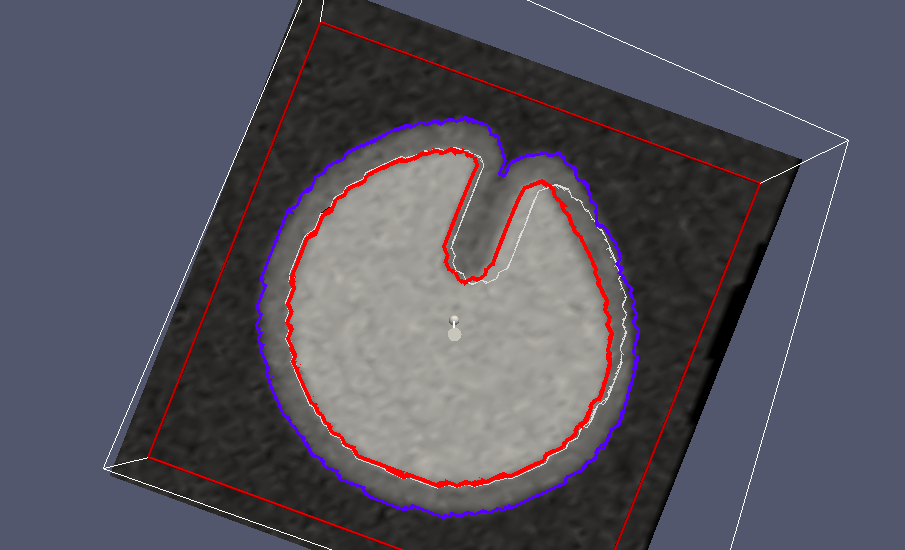
\includegraphics[width=1.0\textwidth]{model2result}
\caption{Result of the segmentation performance on the first
model. In red and blue colors the obtained \ac{wm}/\ac{gm} 
and \ac{gm}/\ac{csf} contours for the deformed image, respectively.
In white color, the initial shape priors for the \ac{wm}/\ac{gm}
interface.
{\color{red}{This figure is to be replaced by the real result,
this is a proof of concept of registration that does not solve
the pv problem. The current figure also removes the outer prior}}}
\label{fig:sulcusmodel_result}
\end{figure}


\subsection{Simulated diffusion data}
%
The proposed method successfully reverted the synthetic distortion
field we applied to the data. With 16x16x16 control points, the
displacements field is dense enough to correctly represent the
synthetic field. Second row in \autoref{fig:fa} shows the fitted
contours obtained by using the original surfaces of the model
as shape priors, with a constant translation of (5.0mm,10mm.,-5.0mm)
to illustrate briefly the extent of the capture range of the algorithm.
Computation time in this case was around 4 minutes in the previously
described platform. \\
%

\begin{figure}
\begin{tabular}{ccccc}
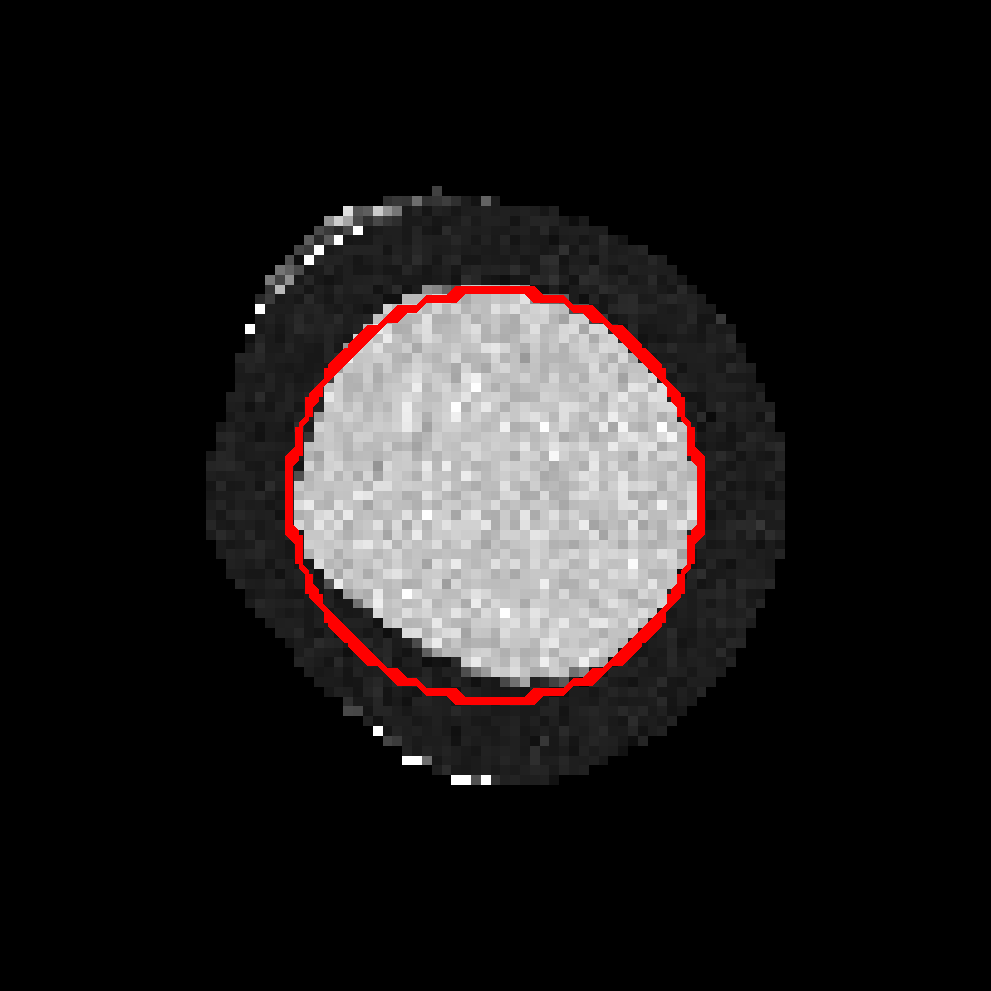
\includegraphics[width=0.19\textwidth]{model1result_b_1} &
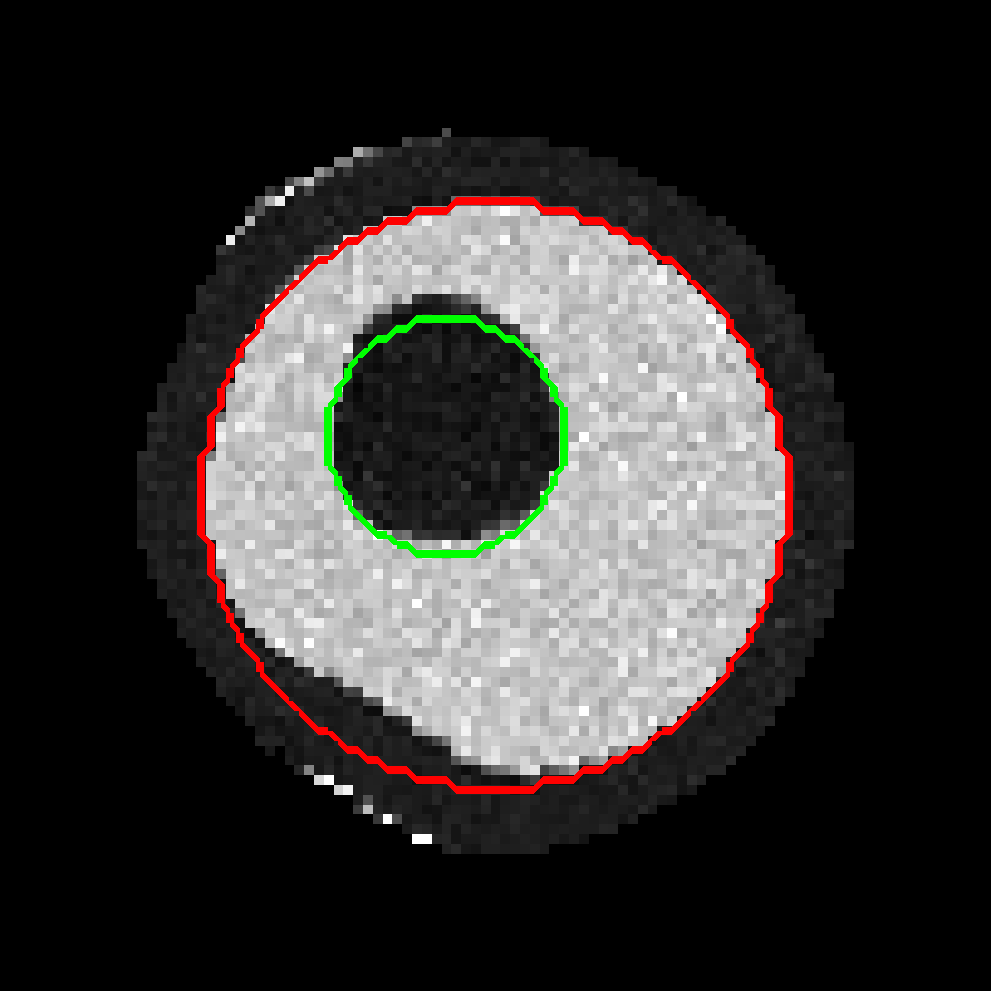
\includegraphics[width=0.19\textwidth]{model1result_b_2} &
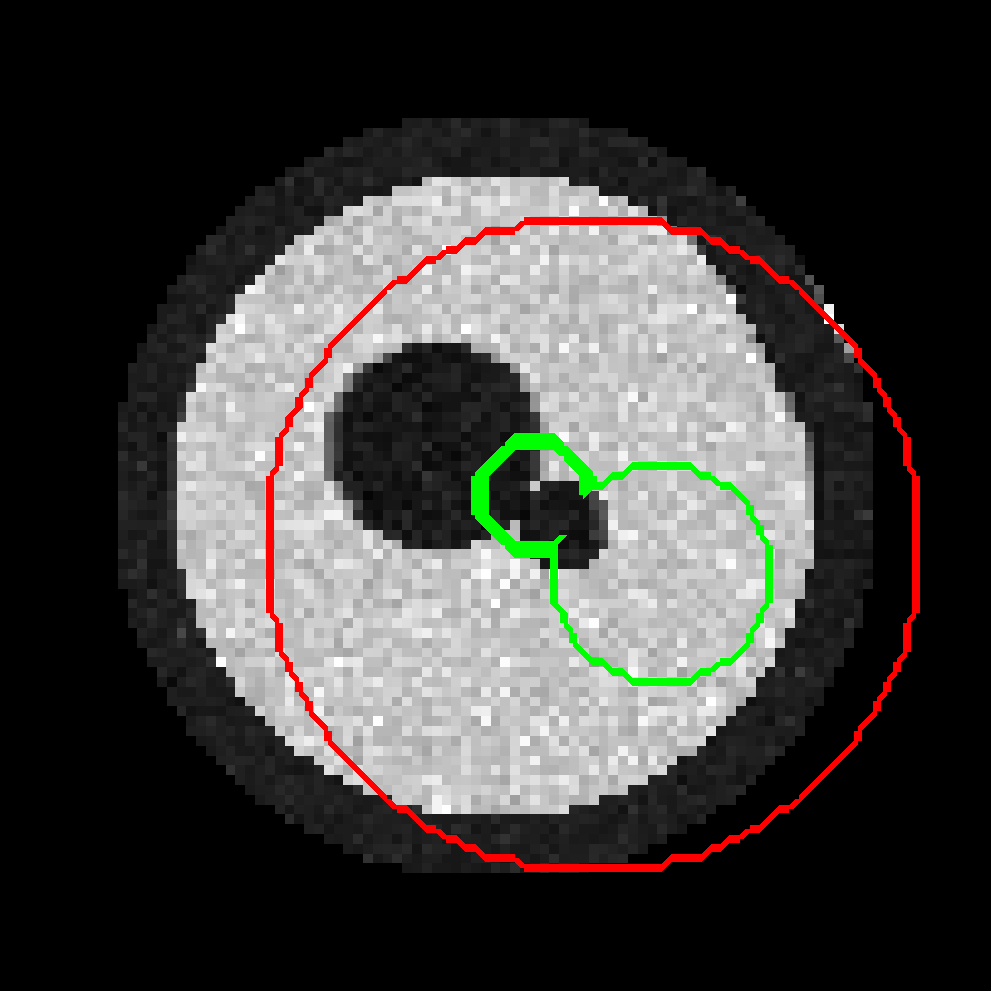
\includegraphics[width=0.19\textwidth]{model1result_b_3} &
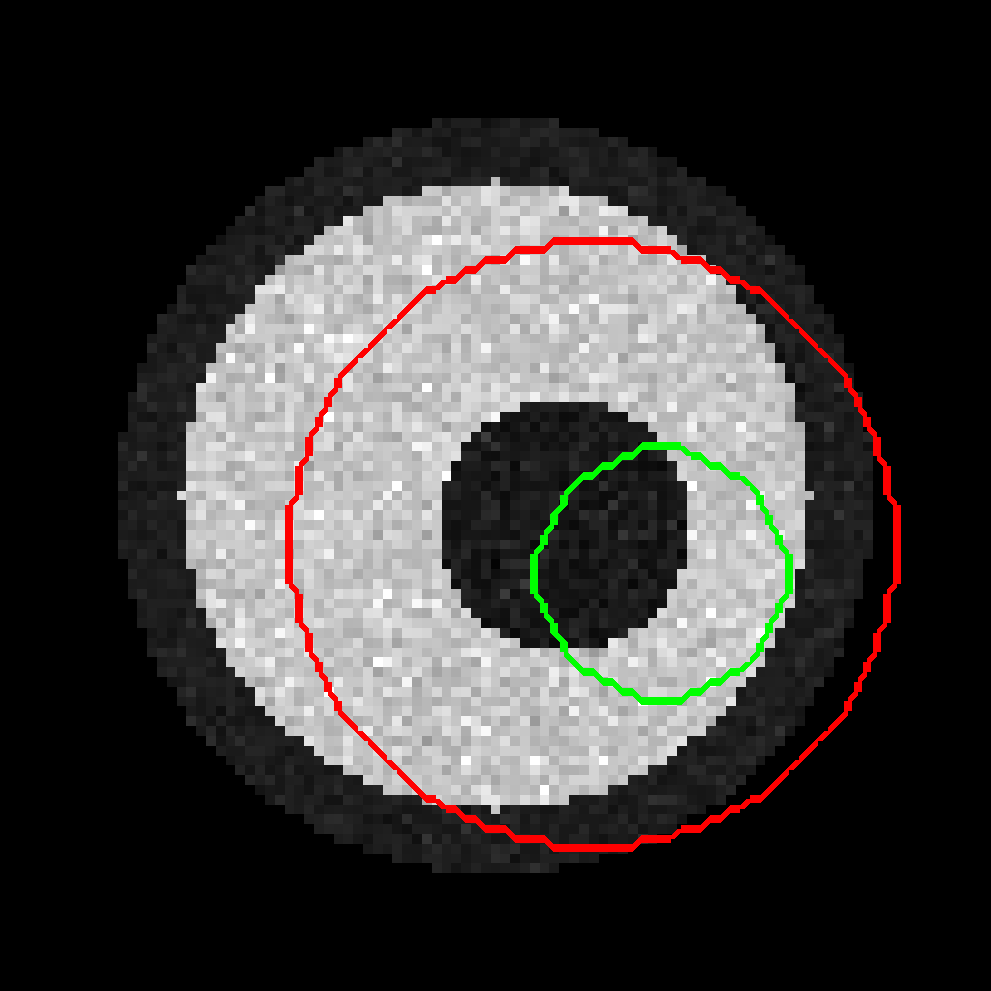
\includegraphics[width=0.19\textwidth]{model1result_b_4} &
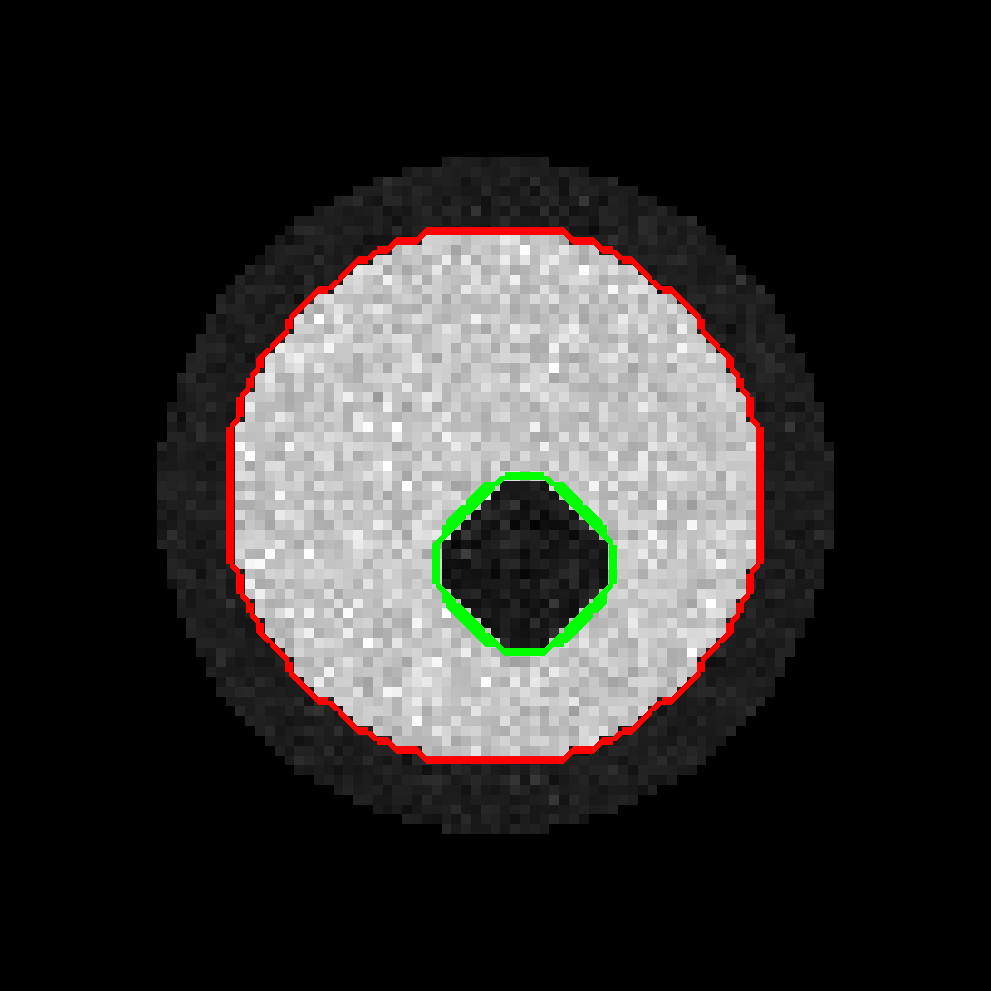
\includegraphics[width=0.19\textwidth]{model1result_b_5} \\
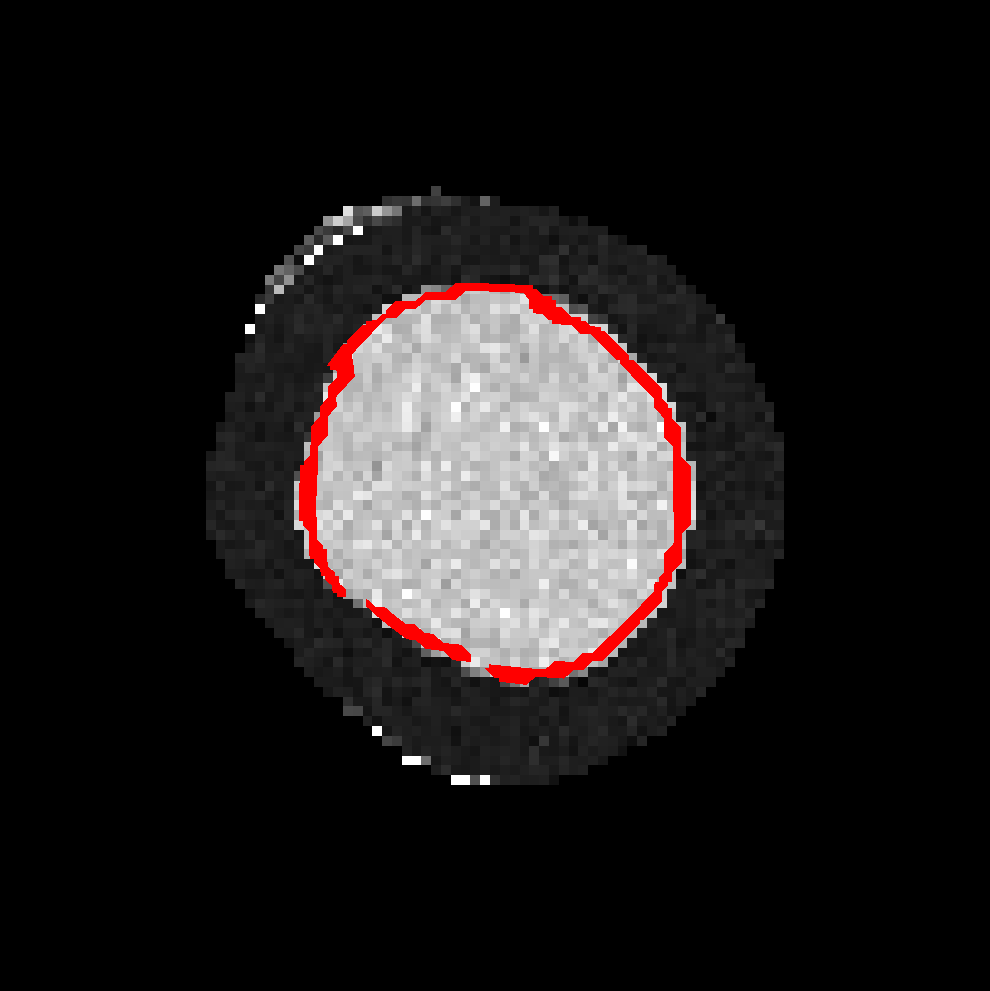
\includegraphics[width=0.19\textwidth]{model1result_a_1} &
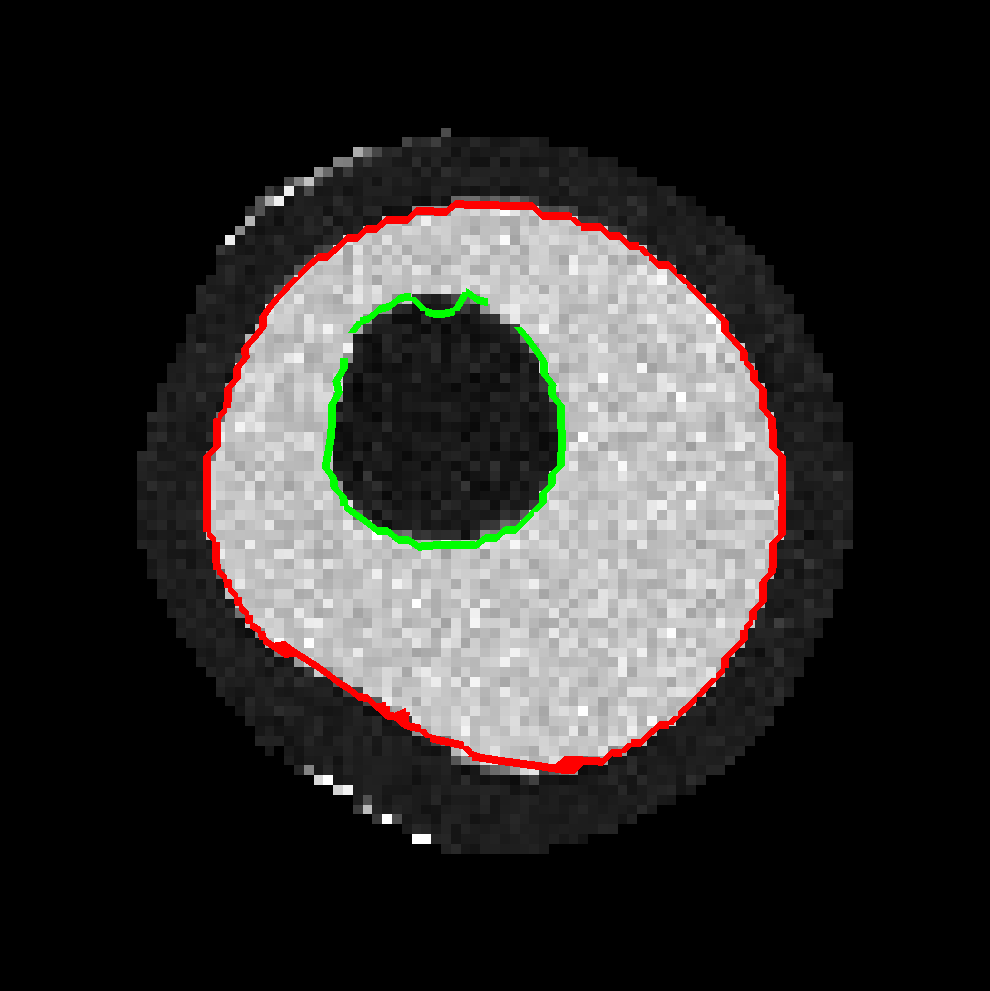
\includegraphics[width=0.19\textwidth]{model1result_a_2} &
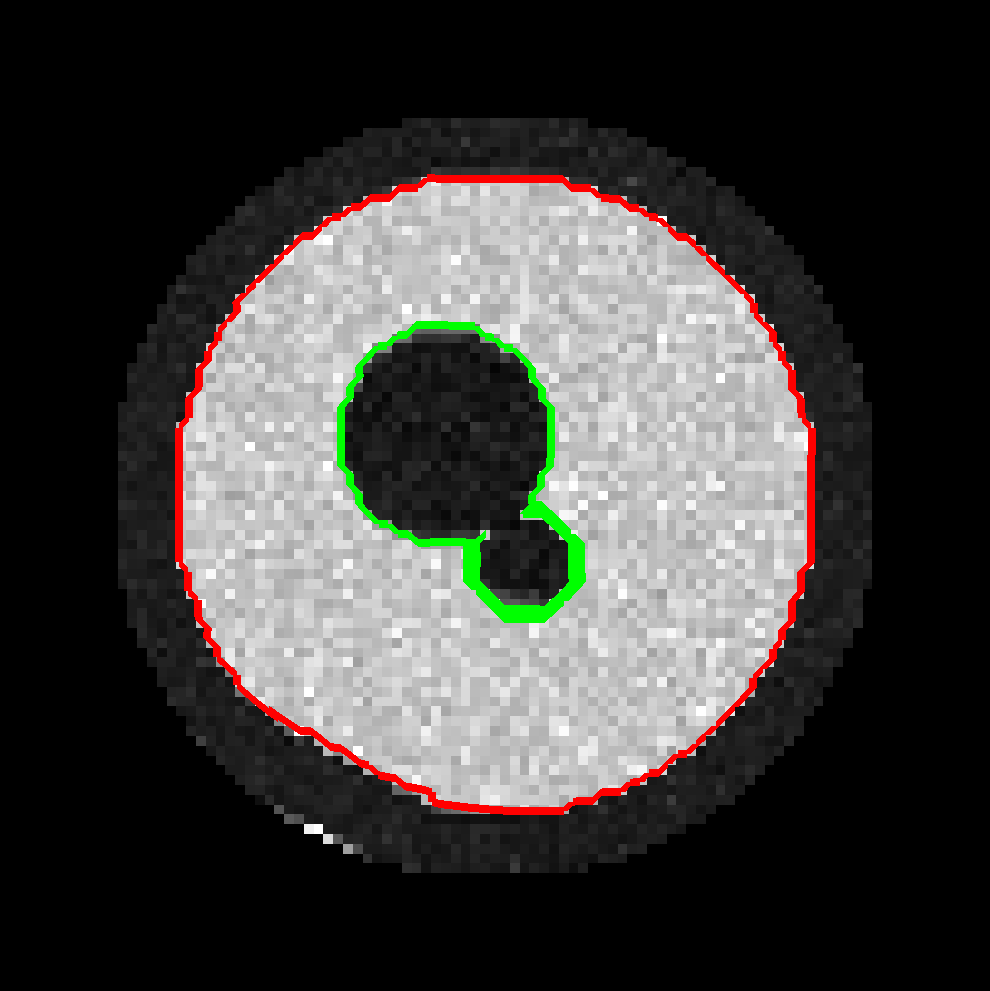
\includegraphics[width=0.19\textwidth]{model1result_a_3} &
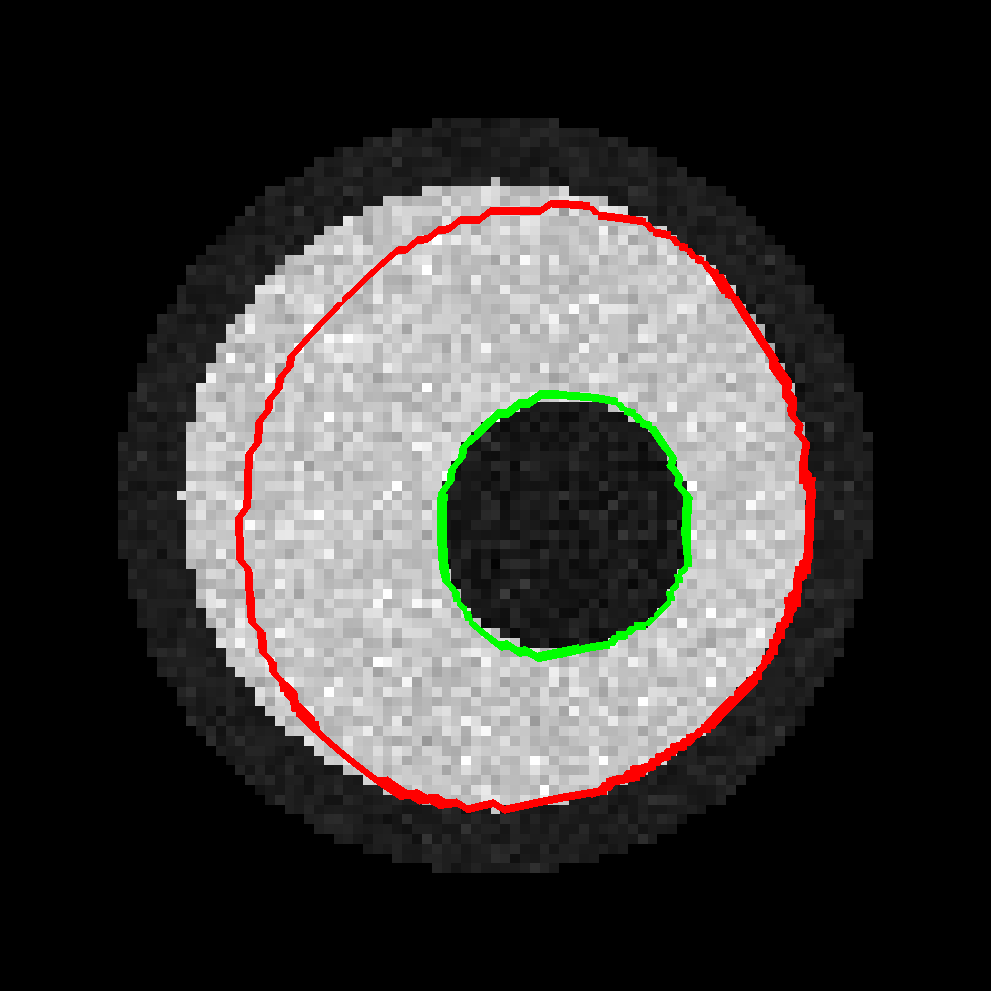
\includegraphics[width=0.19\textwidth]{model1result_a_4} &
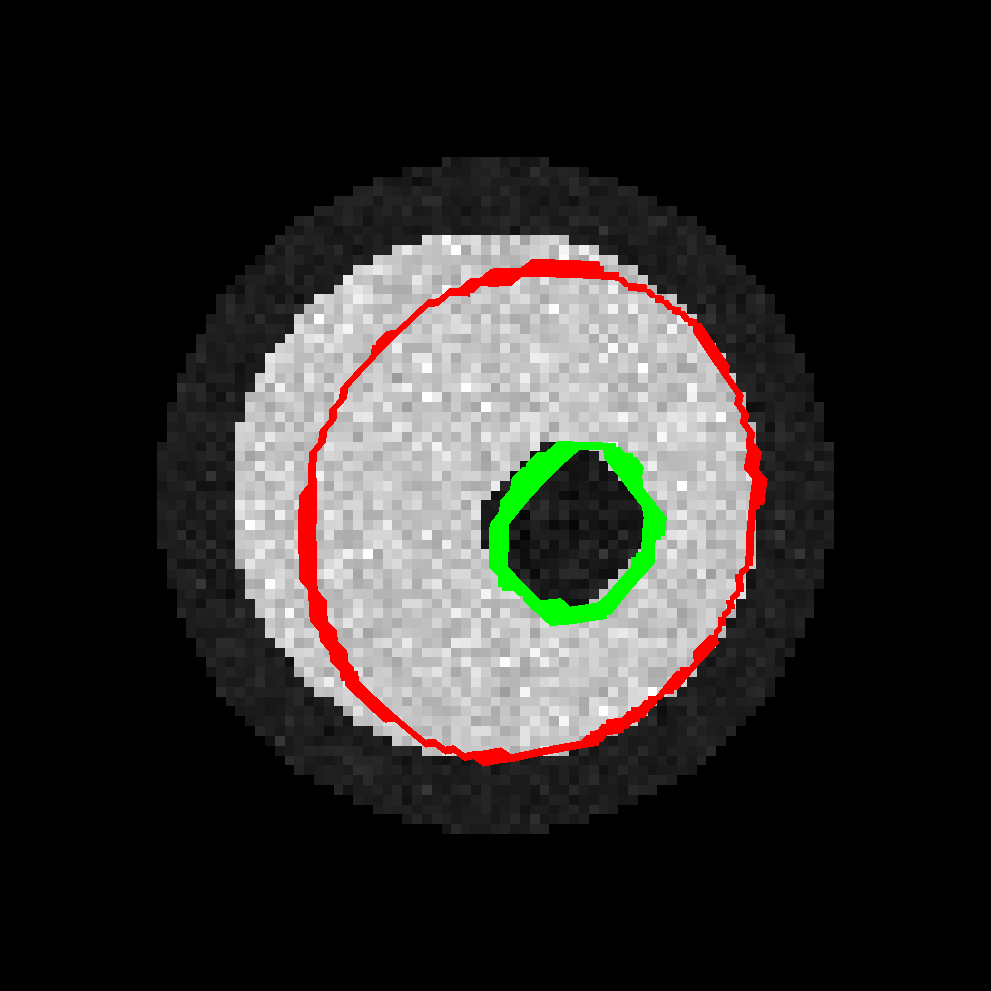
\includegraphics[width=0.19\textwidth]{model1result_a_5} \\
\end{tabular}
\caption{First row presents several slices along Z axis of the distorted \ac{fa} map and
the undistorted \ac{wm}-\ac{gm} and \ac{wm}-\ac{csf} contours given as shape priors. Second row contains the same map, now with the contours after joint segmentation-registration.}
\label{fig:fa}
\end{figure}

\section{Conclusion}
\label{sec:conclusion}
%


%\section{Acknowledgments}
%
The authors gratefully acknowledge V. Estellers for critical discussions at early stages of this project and L. Vese for her generous support.
Further, O. Esteban is supported by .... D. Zosso is supported by the Swiss National Science Foundation (SNF) under grant PBELP2-137727. 


\bibliography{99-References}

\end{document}